\documentclass[10pt]{article}
\usepackage[polish]{babel}
\usepackage[utf8]{inputenc}
\usepackage[T1]{fontenc}
\usepackage{graphicx}
\usepackage[export]{adjustbox}
\graphicspath{ {./images/} }
\usepackage{amsmath}
\usepackage{amsfonts}
\usepackage{amssymb}
\usepackage[version=4]{mhchem}
\usepackage{stmaryrd}
\usepackage{multirow}

\title{EGZAMIN MATURALNY \\
 Z MATEMATYKI \\
 POZIOM ROZSZERZONY }

\author{}
\date{}


\begin{document}
\maketitle
\begin{center}

\includegraphics[max width=\textwidth]{2024_11_21_2d534ae2f00d3e946629g-01}
\end{center}

MAJ 2013

\begin{enumerate}
  \item Sprawdź, czy arkusz egzaminacyjny zawiera 20 stron (zadania 1 - 12). Ewentualny brak zgłoś
\end{enumerate}

Czas pracy: 180 minut

Liczba punktów do uzyskania: 50

MMA-R1\_1P-132

\section*{Zadanie 1. (4 pkt)}
Rozwiąż nierówność \(|2 x-5|-|x+4| \leq 2-2 x\).\\

\includegraphics[max width=\textwidth, center]{2024_11_21_2d534ae2f00d3e946629g-02}

Odpowiedź:

Zadanie 2. (4 pkt)\\
Trapez równoramienny \(A B C D\) o podstawach \(A B\) i \(C D\) jest opisany na okręgu o promieniu \(r\). Wykaż, że \(4 r^{2}=|A B| \cdot|C D|\).\\

\includegraphics[max width=\textwidth, center]{2024_11_21_2d534ae2f00d3e946629g-03}

\begin{center}
\begin{tabular}{|c|l|c|c|}
\hline
\multirow{2}{*}{\begin{tabular}{c}
Wypelnia \\
egzaminator \\
\end{tabular}} & Nr zadania & 1. & 2. \\
\cline { 2 - 4 }
 & Maks. liczba pkt & 4 & 4 \\
\cline { 2 - 4 }
 & Uzyskana liczba pkt &  &  \\
\hline
\end{tabular}
\end{center}

\section*{Zadanie 3. (3 pkt)}
Oblicz, ile jest liczb naturalnych sześciocyfrowych, w zapisie których występuje dokładnie trzy razy cyfra 0 i dokładnie raz wystequje cyfra 5.\\

\includegraphics[max width=\textwidth, center]{2024_11_21_2d534ae2f00d3e946629g-04}\\

\includegraphics[max width=\textwidth, center]{2024_11_21_2d534ae2f00d3e946629g-05}

Odpowiedź:

\begin{center}
\begin{tabular}{|c|l|c|}
\hline
\multirow{3}{*}{\begin{tabular}{l}
Wypetnia \\
egzaminator \\
\end{tabular}} & Nr zadania & 3. \\
\cline { 2 - 3 }
 & Maks. liczba pkt & 3 \\
\cline { 2 - 3 }
 & Uzyskana liczba pkt &  \\
\hline
\end{tabular}
\end{center}

\section*{Zadanie 4. (4 pkt)}
Rozwiąż równanie \(\cos 2 x+\cos x+1=0\) dla \(x \in\langle 0,2 \pi\rangle\).\\

\includegraphics[max width=\textwidth, center]{2024_11_21_2d534ae2f00d3e946629g-06}

Odpowiedź:

\section*{Zadanie 5. (5 pkt)}
Ciag liczbowy \((a, b, c)\) jest arytmetyczny i \(a+b+c=33\), natomiast ciag \((a-1, b+5, c+19)\) jest geometryczny. Oblicz \(a, b, c\).\\

\includegraphics[max width=\textwidth, center]{2024_11_21_2d534ae2f00d3e946629g-07}

Odpowiedź:

\begin{center}
\begin{tabular}{|c|l|c|c|}
\hline
\multirow{2}{*}{\begin{tabular}{c}
Wypełnia \\
egzaminator \\
\end{tabular}} & Nr zadania & 4. & 5. \\
\cline { 2 - 4 }
 & Maks. liczba pkt & 4 & 5 \\
\cline { 2 - 4 }
 & Uzyskana liczba pkt &  &  \\
\hline
\end{tabular}
\end{center}

\section*{Zadanie 6. (6 pkt)}
Wyznacz wszystkie wartości parametru \(m\), dla których równanie \(x^{2}+2(1-m) x+m^{2}-m=0\) ma dwa różne rozwiązania rzeczywiste \(x_{1}, x_{2}\) spełniające warunek \(x_{1} \cdot x_{2} \leq 6 m \leq x_{1}^{2}+x_{2}^{2}\).

\begin{center}
\begin{tabular}{|c|c|c|c|c|c|c|c|c|c|c|c|c|c|c|c|c|c|c|c|c|c|c|}
\hline
 &  &  &  &  &  &  &  &  &  &  &  &  &  &  &  &  &  &  &  &  &  &  \\
\hline
 &  &  &  &  &  &  &  &  &  &  &  &  &  &  &  &  &  &  &  &  &  &  \\
\hline
 &  &  &  &  &  &  &  &  &  &  &  &  &  &  &  &  &  &  &  &  &  &  \\
\hline
 &  &  &  &  &  &  &  &  &  &  &  &  &  &  &  &  &  &  &  &  &  &  \\
\hline
 &  &  &  &  &  &  &  &  &  &  &  &  &  &  &  &  &  &  &  &  &  &  \\
\hline
 &  &  &  &  &  &  &  &  &  &  &  &  &  &  &  &  &  &  &  &  &  &  \\
\hline
 &  &  &  &  &  &  &  &  &  &  &  &  &  &  &  &  &  &  &  &  &  &  \\
\hline
 &  &  &  &  &  &  &  &  &  &  &  &  &  &  &  &  &  &  &  &  &  &  \\
\hline
 &  &  &  &  &  &  &  &  &  &  &  &  &  &  &  &  &  &  &  &  &  &  \\
\hline
 &  &  &  &  &  &  &  &  &  &  &  &  &  &  &  &  &  &  &  &  &  &  \\
\hline
 &  &  &  &  &  &  &  &  &  &  &  &  &  &  &  &  &  &  &  &  &  &  \\
\hline
 &  &  &  &  &  &  &  &  &  &  &  &  &  &  &  &  &  &  &  &  &  &  \\
\hline
 &  &  &  &  &  &  &  &  &  &  &  &  &  &  &  &  &  &  &  &  &  &  \\
\hline
 &  &  &  &  &  &  &  &  &  &  &  &  &  &  &  &  &  &  &  &  &  &  \\
\hline
 &  &  &  &  &  &  &  &  &  &  &  &  &  &  &  &  &  &  &  &  &  &  \\
\hline
 &  &  &  &  &  &  &  &  &  &  &  &  &  &  &  &  &  &  &  &  &  &  \\
\hline
 &  &  &  &  &  &  &  &  &  &  &  &  &  &  &  &  &  &  &  &  &  &  \\
\hline
 &  &  &  &  &  &  &  &  &  &  &  &  &  &  &  &  &  &  &  &  &  &  \\
\hline
 &  &  &  &  &  &  &  &  &  &  &  &  &  &  &  &  &  &  &  &  &  &  \\
\hline
 &  &  &  &  &  &  &  &  &  &  &  &  &  &  &  &  &  &  &  &  &  &  \\
\hline
 &  &  &  &  &  &  &  &  &  &  &  &  &  &  &  &  &  &  &  &  &  &  \\
\hline
 &  &  &  &  &  &  &  &  &  &  &  &  &  &  &  &  &  &  &  &  &  &  \\
\hline
 &  &  &  &  &  &  &  &  &  &  &  &  &  &  &  &  &  &  &  &  &  &  \\
\hline
 &  &  &  &  &  &  &  &  &  &  &  &  &  &  &  &  &  &  &  &  &  &  \\
\hline
 &  &  &  &  &  &  &  &  &  &  &  &  &  &  &  &  &  &  &  &  &  &  \\
\hline
 &  &  &  &  &  &  &  &  &  &  &  &  &  &  &  &  &  &  &  &  &  &  \\
\hline
 &  &  &  &  &  &  &  &  &  &  &  &  &  &  &  &  &  &  &  &  &  &  \\
\hline
 &  &  &  &  &  &  &  &  &  &  &  &  &  &  &  &  &  &  &  &  &  &  \\
\hline
 &  &  &  &  &  &  &  &  &  &  &  &  &  &  &  &  &  &  &  &  &  &  \\
\hline
 &  &  &  &  &  &  &  &  &  &  &  &  &  &  &  &  &  &  &  &  &  &  \\
\hline
 &  &  &  &  &  &  &  &  &  &  &  &  &  &  &  &  &  &  &  &  &  &  \\
\hline
 &  &  &  &  &  &  &  &  &  &  &  &  &  &  &  &  &  &  &  &  &  &  \\
\hline
 &  &  &  &  &  &  &  &  &  &  &  &  &  &  &  &  &  &  &  &  &  &  \\
\hline
 &  &  &  &  &  &  &  &  &  &  &  &  &  &  &  &  &  &  &  &  &  &  \\
\hline
 &  &  &  &  &  &  &  &  &  &  &  &  &  &  &  &  &  &  &  &  &  &  \\
\hline
 &  &  &  &  &  &  &  &  &  &  &  &  &  &  &  &  &  &  &  &  &  &  \\
\hline
 &  &  &  &  &  &  &  &  &  &  &  &  &  &  &  &  &  &  &  &  &  &  \\
\hline
 &  &  &  &  &  &  &  &  &  &  &  &  &  &  &  &  &  &  &  &  &  &  \\
\hline
 &  &  &  &  &  &  &  &  &  &  &  &  &  &  &  &  &  &  &  &  &  &  \\
\hline
 &  &  &  &  &  &  &  &  &  &  &  &  &  &  &  &  &  &  &  &  &  &  \\
\hline
 &  &  &  &  &  &  &  &  &  &  &  &  &  &  &  &  &  &  &  &  &  &  \\
\hline
 &  &  &  &  &  &  &  &  &  &  &  &  &  &  &  &  &  &  &  &  &  &  \\
\hline
 &  &  &  &  &  &  &  &  &  &  &  &  &  &  &  &  &  &  &  &  &  &  \\
\hline
 &  &  &  &  &  &  &  &  &  &  &  &  &  &  &  &  &  &  &  &  &  &  \\
\hline
\end{tabular}
\end{center}

\begin{center}

\includegraphics[max width=\textwidth]{2024_11_21_2d534ae2f00d3e946629g-09}
\end{center}

Odpowiedź:

\begin{center}
\begin{tabular}{|c|l|c|}
\hline
\multirow{2}{*}{\begin{tabular}{l}
Wypetnia \\
egzaminator \\
\end{tabular}} & Nr zadania & \(\mathbf{6}\). \\
\cline { 2 - 3 }
 & Maks. liczba pkt & \(\mathbf{6}\) \\
\cline { 2 - 3 }
 & Uzyskana liczba pkt &  \\
\hline
\end{tabular}
\end{center}

\section*{Zadanie 7. (4 pkt)}
Prosta o równaniu \(3 x-4 y-36=0\) przecina okrag o środku \(S=(3,12)\) w punktach \(A\) i \(B\). Długość odcinka \(A B\) jest równa 40. Wyznacz równanie tego okręgu.\\

\includegraphics[max width=\textwidth, center]{2024_11_21_2d534ae2f00d3e946629g-10}\\

\includegraphics[max width=\textwidth, center]{2024_11_21_2d534ae2f00d3e946629g-11}

Odpowiedź:

\begin{center}
\begin{tabular}{|c|l|c|}
\hline
\multirow{2}{*}{\begin{tabular}{l}
Wypelnia \\
egzaminator \\
\end{tabular}} & Nr zadania & 7. \\
\cline { 2 - 3 }
 & Maks. liczba pkt & 4 \\
\cline { 2 - 3 }
 & Uzyskana liczba pkt &  \\
\hline
\end{tabular}
\end{center}

\section*{Zadanie 8. (4 pkt)}
Reszta z dzielenia wielomianu \(W(x)=4 x^{3}-5 x^{2}-23 x+m\) przez dwumian \(x+1\) jest równa 20 . Oblicz wartość współczynnika \(m\) oraz pierwiastki tego wielomianu.\\

\includegraphics[max width=\textwidth, center]{2024_11_21_2d534ae2f00d3e946629g-12}

Odpowiedź:

Zadanie 9. (5 pkt)\\
Dany jest trójkąt \(A B C\), w którym \(|A C|=17\) i \(|B C|=10\). Na boku \(A B\) leży punkt \(D\) taki, że \(|A D|:|D B|=3: 4\) oraz \(|D C|=10\). Oblicz pole trójkąta \(A B C\).\\

\includegraphics[max width=\textwidth, center]{2024_11_21_2d534ae2f00d3e946629g-13}

Odpowiedź:

\begin{center}
\begin{tabular}{|c|l|c|c|}
\hline
\multirow{2}{*}{\begin{tabular}{c}
Wypelnia \\
egzaminator \\
\end{tabular}} & Nr zadania & 8. & 9. \\
\cline { 2 - 4 }
 & Maks. liczba pkt & 4 & 5 \\
\cline { 2 - 4 }
 & Uzyskana liczba pkt &  &  \\
\hline
\end{tabular}
\end{center}

\section*{Zadanie 10. (4 pkt)}
W ostrosłupie \(A B C S\) podstawa \(A B C\) jest trójkątem równobocznym o boku długości \(a\). Krawędź \(A S\) jest prostopadła do płaszczyzny podstawy. Odległość wierzchołka \(A\) od ściany \(B C S\) jest równa \(d\). Wyznacz objętość tego ostrosłupa.\\

\includegraphics[max width=\textwidth, center]{2024_11_21_2d534ae2f00d3e946629g-14}\\

\includegraphics[max width=\textwidth, center]{2024_11_21_2d534ae2f00d3e946629g-15}

Odpowiedź:

\begin{center}
\begin{tabular}{|c|l|c|}
\hline
\multirow{2}{*}{\begin{tabular}{l}
Wypelnia \\
egzaminator \\
\end{tabular}} & Nr zadania & 10. \\
\cline { 2 - 3 }
 & Maks. liczba pkt & 4 \\
\cline { 2 - 3 }
 & Uzyskana liczba pkt &  \\
\hline
\end{tabular}
\end{center}

\section*{Zadanie 11. (4 pkt)}
Rzucamy cztery razy symetryczną sześcienną kostką do gry. Oblicz prawdopodobieństwo zdarzenia polegajacego na tym, że iloczyn liczb oczek otrzymanych we wszystkich czterech rzutach będzie równy 60 .\\

\includegraphics[max width=\textwidth, center]{2024_11_21_2d534ae2f00d3e946629g-16}\\

\includegraphics[max width=\textwidth, center]{2024_11_21_2d534ae2f00d3e946629g-17}

Odpowiedź:

\begin{center}
\begin{tabular}{|c|l|c|}
\hline
\multirow{2}{*}{\begin{tabular}{c}
Wypelnia \\
egzaminator \\
\end{tabular}} & Nr zadania & 11. \\
\cline { 2 - 3 }
 & Maks. liczba pkt & 4 \\
\cline { 2 - 3 }
 & Uzyskana liczba pkt &  \\
\hline
\end{tabular}
\end{center}

\section*{Zadanie 12. (3 pkt)}
Na rysunku przedstawiony jest fragment wykresu funkcji logarytmicznej \(f\) określonej wzorem \(f(x)=\log _{2}(x-p)\).\\
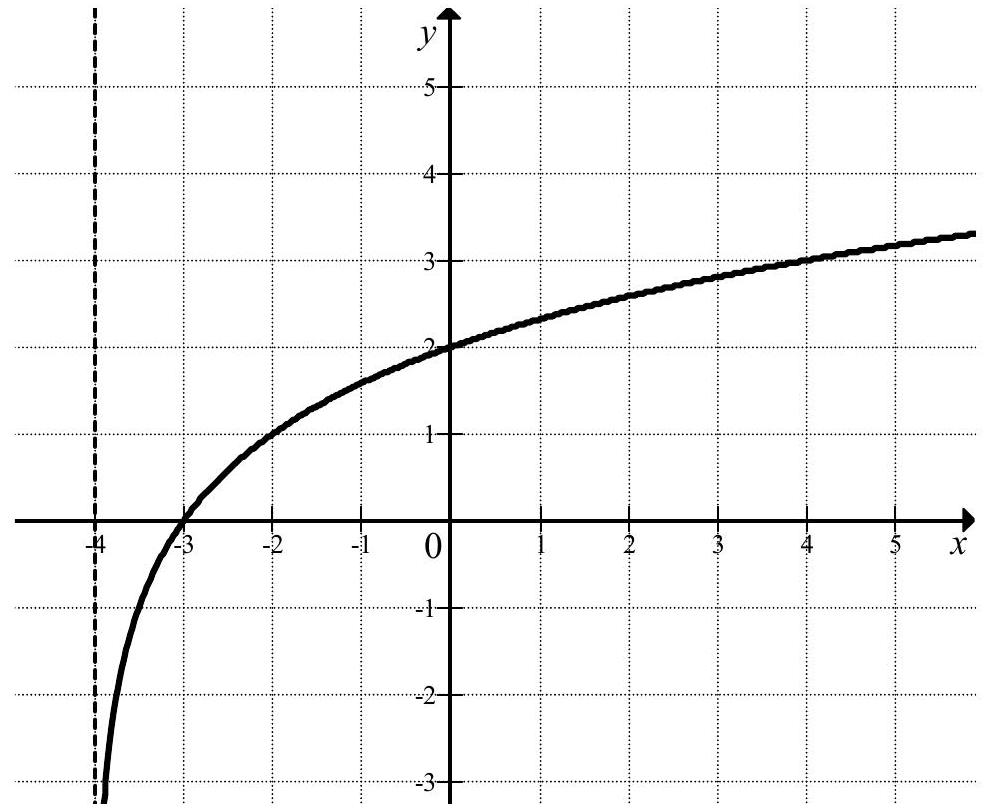
\includegraphics[max width=\textwidth, center]{2024_11_21_2d534ae2f00d3e946629g-18}\\
a) Podaj wartość \(p\).\\
b) Narysuj wykres funkcji określonej wzorem \(y=|f(x)|\).\\
c) Podaj wszystkie wartości parametru \(m\), dla których równanie \(|f(x)|=m\) ma dwa rozwiazzania o przeciwnych znakach.\\

\includegraphics[max width=\textwidth, center]{2024_11_21_2d534ae2f00d3e946629g-18(1)}\\

\includegraphics[max width=\textwidth, center]{2024_11_21_2d534ae2f00d3e946629g-19}

Odpowiedź:

\begin{center}
\begin{tabular}{|c|l|c|}
\hline
\multirow{2}{*}{\begin{tabular}{c}
Wypelnia \\
egzaminator \\
\end{tabular}} & Nr zadania & 12. \\
\cline { 2 - 3 }
 & Maks. liczba pkt & 3 \\
\cline { 2 - 3 }
 & Uzyskana liczba pkt &  \\
\hline
\end{tabular}
\end{center}

\section*{BRUDNOPIS}

\end{document}